\documentclass[xcolor=table]{beamer}
\usepackage{fontspec}
\usepackage{natbib}
\usepackage{gb4e} 
\usepackage[table]{xcolor}
\usepackage{booktabs} 
%\usepackage{color}
\usepackage{graphicx}
\usepackage{tikz}
\usetikzlibrary{trees}
\usepackage{bibentry}

% \setmainfont[Mapping=tex-text]{Charis SIL}
\let\sfdefault\rmdefault
%\newcommand{\racine}[1]{\begin{math}\sqrt{#1}\end{math}} 
\newfontfamily\phon[Mapping=tex-text,Ligatures=Common,Scale=MatchLowercase,FakeSlant=0.3]{Charis SIL} 
\newcommand{\ipa}[1]{{\phon \mbox{#1}}} %API tjs en italique
\newcommand{\grise}[1]{\cellcolor{lightgray}\textbf{#1}} 
\newcommand{\ra}{$\Sigma_1$} 
\newcommand{\rc}{$\Sigma_3$} 
\newcommand{\ro}{$\Sigma$} 
 \begin{document}



 \title{Vers un nouvel outil d'annotation de textes et de traitement de données lexicographiques pour les langues à tradition orale\\Axe 6 - Opération LR2.5}
 \author{Guillaume Jacques}
 \maketitle


 \begin{frame} 
 \frametitle{ }
 \begin{enumerate}%[<+->]
 \item Membres: Guillaume Jacques (CRLAO), Benoît Sagot (Alpage), Christian Chanard (LLACAN), Céline Buret (LACITO), Thomas Pellard (CRLAO)
 \item Recrutement de Rémy Bonnet (1er juin 2015, contrat de trois ans)
  \begin{itemize}
\item Besoins des linguistes de terrain
\item Outils d'analyse morphologique
\item ANR HimalCo
 \end{itemize}
 \end{enumerate}

\end{frame}

 \begin{frame} 
 \frametitle{I. Besoins des linguistes de terrain}
  Insuffisances de Toolbox 
 \begin{itemize}
 \item Analyseur morphologique insuffisant pour traiter les langues à morphologie lourde
 \item Absence d'analyseur syntaxique
 \item Absence de contrôle de cohérence de la structure des données lexicales
 \end{itemize}
\end{frame}

 \begin{frame} 
 \frametitle{I. Besoins des linguistes de terrain}
 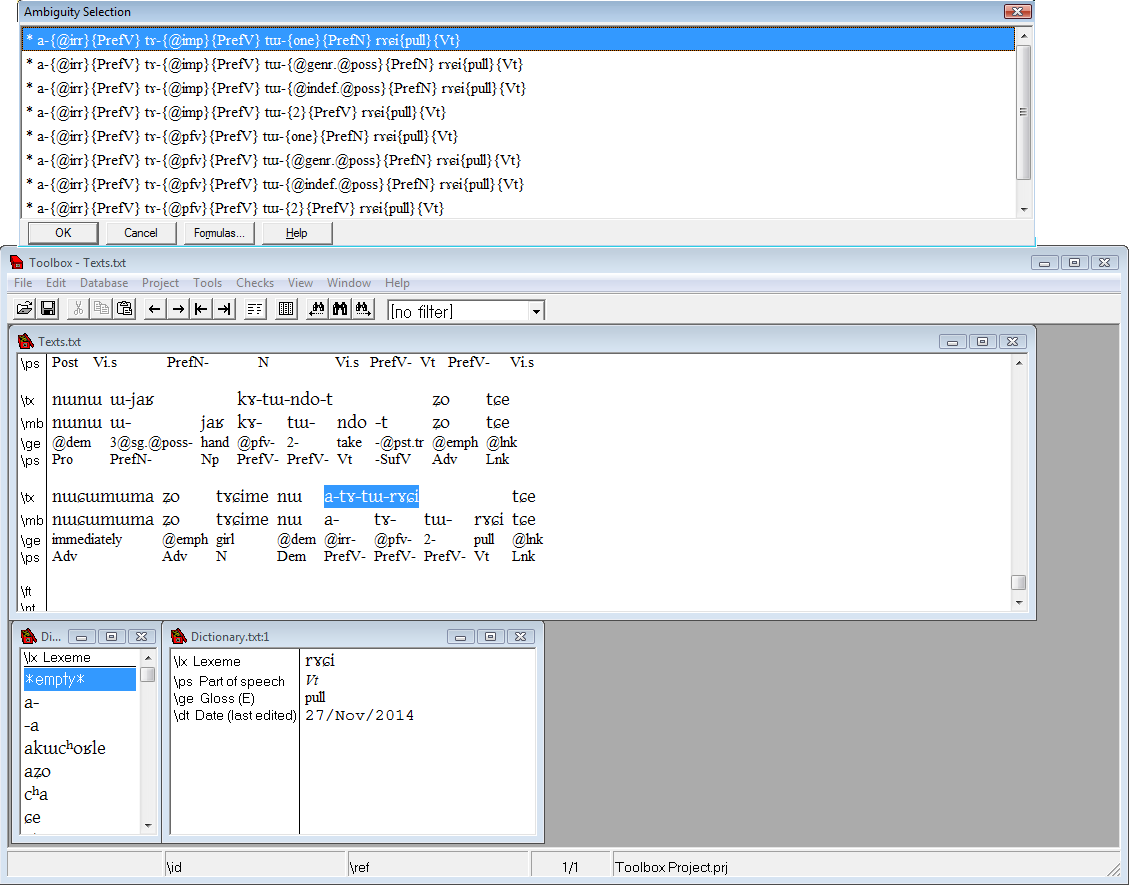
\includegraphics[width=\textwidth]{toolbox-ex.png}
\end{frame}
 \begin{frame} 
 \frametitle{I. Besoins des linguistes de terrain}
 \begin{itemize}
 \item Outil multi-plateforme au code ouvert
 \item Analyseur/générateur morphologique (transducteur amélioré)
 \item Analyseur syntaxique simple
 \item Démocratisation des outils développés de la linguistique quantitative auprès des linguistes de terrains
  \end{itemize}
\end{frame}


 \begin{frame} 
 \frametitle{II. Outils déjà disponibles}
     \bibliographystyle{unified}
  \nobibliography{bibliogj.bib}
 \begin{itemize}
 \item Analyseur/générateur morphologique 
 \item Exemple d'application (sur le Khaling):
 \item \bibentry{walther14compactness}
 \item Pas d'interface graphique, peu accessible aux linguistes non-formalistes
  \end{itemize} 
\end{frame}

  
 \begin{frame} 
 \frametitle{III. Projet ANR Corpus HimalCo (2015-2016)}
 \begin{enumerate}%[<+->]
 \item Membres: Guillaume Jacques, Alexis Michaud, Aimée Lahaussois, Séverine 
 Guillaume, Céline Buret
\item Développement d'une librairie python LMF $\Rightarrow$ HTML, \LaTeX, RTF, interface Android
\item Dictionnaires parlants (japhug, na, khaling)
\item Corpus parallèles (langues kiranties)
\item Site Pangloss
 \end{enumerate}
 
  
\includegraphics[width=0.4\textwidth]{anr.JPG} \centering
  \end{frame}   
  
 \begin{frame} 
 \frametitle{III. Projet ANR Corpus HimalCo}  
   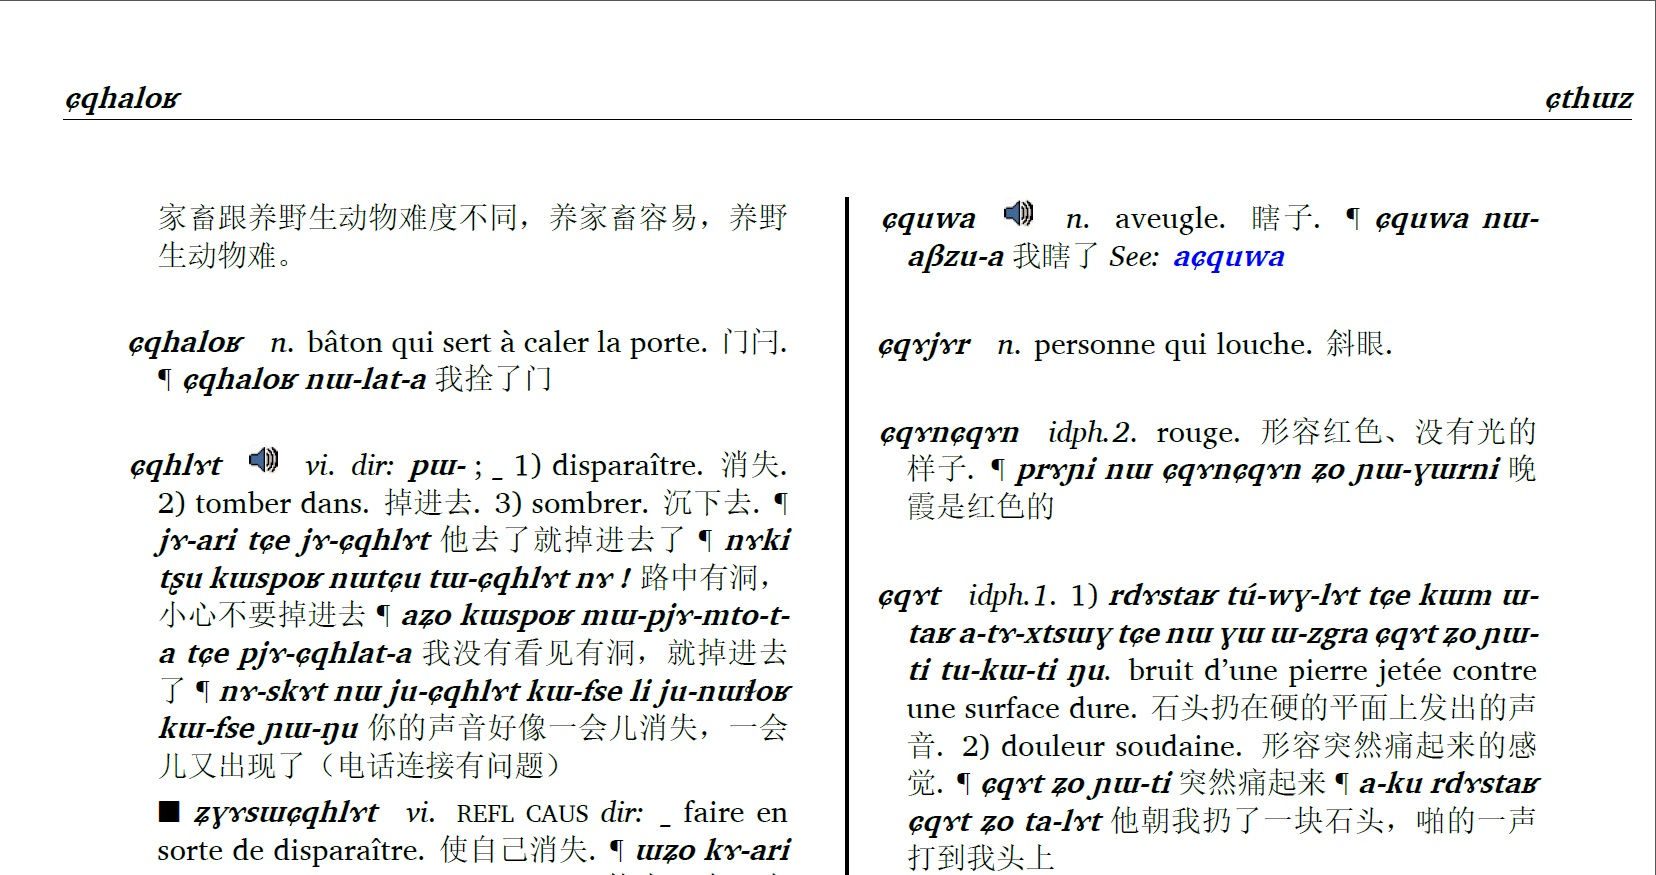
\includegraphics[width=\textwidth]{dico.jpg} \centering
  \end{frame}   
  
 \begin{frame} 
 \frametitle{Conclusion}  
\begin{itemize}
\item Réutilisation des outils déjà développés (transducteur amélioré, librairie Python de traitement de données lexicales)
\item Interface graphique
\item Outil d'exploration morphosyntaxique de corpus, aide à la conception de dictionnaires, de corpus annotés en lignes et de grammaires

\item Vocation à remplacer ses concurrents (Toolbox et FLEX) et à devenir l'outil standard au niveau international.
\end{itemize} 
 
\end{frame}   

\end{document}